\documentclass{article}

\usepackage[utf8]{inputenc}
\usepackage[ngerman]{babel}
\usepackage[ngerman]{translator}
\usepackage[T1]{fontenc}
\usepackage{enumitem}
\usepackage{graphicx}
\usepackage{float}
\usepackage{url}
\usepackage[bottom]{footmisc}
\usepackage{hyperref}
\usepackage[nonumberlist, section=subsection]{glossaries}

\title{\textbf{Entwurf} \\ Cryptographics}
\author{}
\date{\today}

%Glossar-Befehle anschalten
\makeglossaries
% \newglossaryentry{identifier}{name={Name}, description={Description}}

\begin{document}

% The cover page.
\maketitle
\begin{table}[b]
  \begin{tabular}{| l | l | l |}
    \hline
    \textbf{Phase} & \textbf{Verantwortlicher} & \textbf{Email} \\ \hline
    Pflichtenheft & Matthias Jaenicke & matthias.jaenicke@student.kit.edu \\ \hline
    Entwurf & Matthias Plappert & undkc@student.kit.edu \\
            & Julien Duman & uncyc@student.kit.edu \\ \hline
    Implementierung & Christian Dreher & uaeef@student.kit.edu \\ \hline
    Qualitätssicherung & Wasilij Beskorovajnov & uajkm@student.kit.edu \\ \hline
    Präsentation & Aydin Tekin & aydin.tekin@student.kit.edu \\ \hline
    \end{tabular}
\end{table}
\thispagestyle{empty}
\newpage

% Table of contents page.
\tableofcontents
\newpage

% Start of the actual document.
\section{Einleitung}
In diesem Heft werden die Entwürfe zur Implementierung von Cryptographics spezifiziert erläutert.

\section{Aufbau}

\subsection{Architektur}
Die Architektur sieht drei Hierarchieebenen vor. Die erste Ebene, Main-Ebene genannt,
ist dafür verantwortlich, die Controller aus der zweiten Ebene auszutauschen. Controller
zweiten Ebene sind der StartController, der einen Blickfang und eine Übersicht mit der
Zeitlinie darstellt, und der ContainerController, der diejenigen UI-Elemente verwaltet,
die in jedem Verfahren gleich sind. Dabei ist der ContainerController dafür verantwortlich,
die dritte Ebene zu deligieren. Diese Ebene besteht aus Controllern, die ein spezifisches
Verfahren visualisieren und diese Visualisierung verwalten.

\subsection{Klassendiagramm}

\section{Klassenbeschreibung}
  \subsection{Paket edu.kit.iks.Cryptographics}
    \subsubsection{Klasse MainController}
      Der MainController erzeugt das Fenster und verwaltet Start- und VisualizationContainerController.
      \begin{figure}[H]
        \centering
        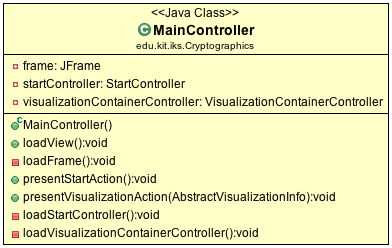
\includegraphics[width=\textwidth]{resources/edu-kit-iks-Cryptographics-MainController}
      \end{figure}

      \textbf{Superklassen und Interfaces}
      \begin{itemize}
        \item edu.kit.iks.CryptographicsLib.AbstractController
      \end{itemize}
      
      \textbf{Methoden}
      \begin{itemize}
        \item public void presentStartAction() \newline
        Läd den StartController und zeigt seine View an.
      \end{itemize}

\subsection{Paket edu.kit.iks.CryptographicsLib}
\subsection{Paket edu.kit.iks.Cryptographics.Vigenere}
\subsection{Paket edu.kit.iks.Cryptographics.Caesar}
\subsection{Paket edu.kit.iks.Cryptographics.DiffieHellman}

\section{Abläufe}

\section{Entwurfdaten}

\section{Anhang}
\glsaddall
\printglossary[numberedsection, style=altlist]

\end{document}
